\section{Tractor Towing Configuration}
The single body dynamics model derivation is based on the current towing configuration and tractor used by the South Pole Traverse. Currently, Caterpillar and AGCO MT865 tractors and a sled system is used. A picture and diagram of the setup are shown in Figures \ref{fig:South_Pole_Traverse_Tractor_and_Sled_Configuration} and \ref{fig:Top_View_Diagram_South_Pole_Traverse} respectively. The sled system consists of four sleds each supporting two, 10,000 kg bladders each. 
\begin{figure}[t]
    \centering
    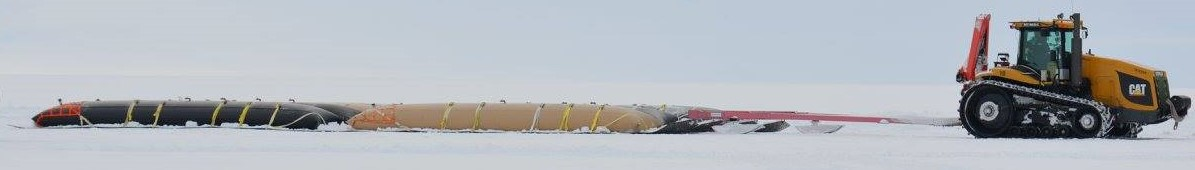
\includegraphics[width= 5.5in]{SPT_Tractor}
    \caption{South Pole Traverse tractor and sled configuration}
    \label{fig:South_Pole_Traverse_Tractor_and_Sled_Configuration}
\end{figure}
\begin{figure}[t]
    \centering
    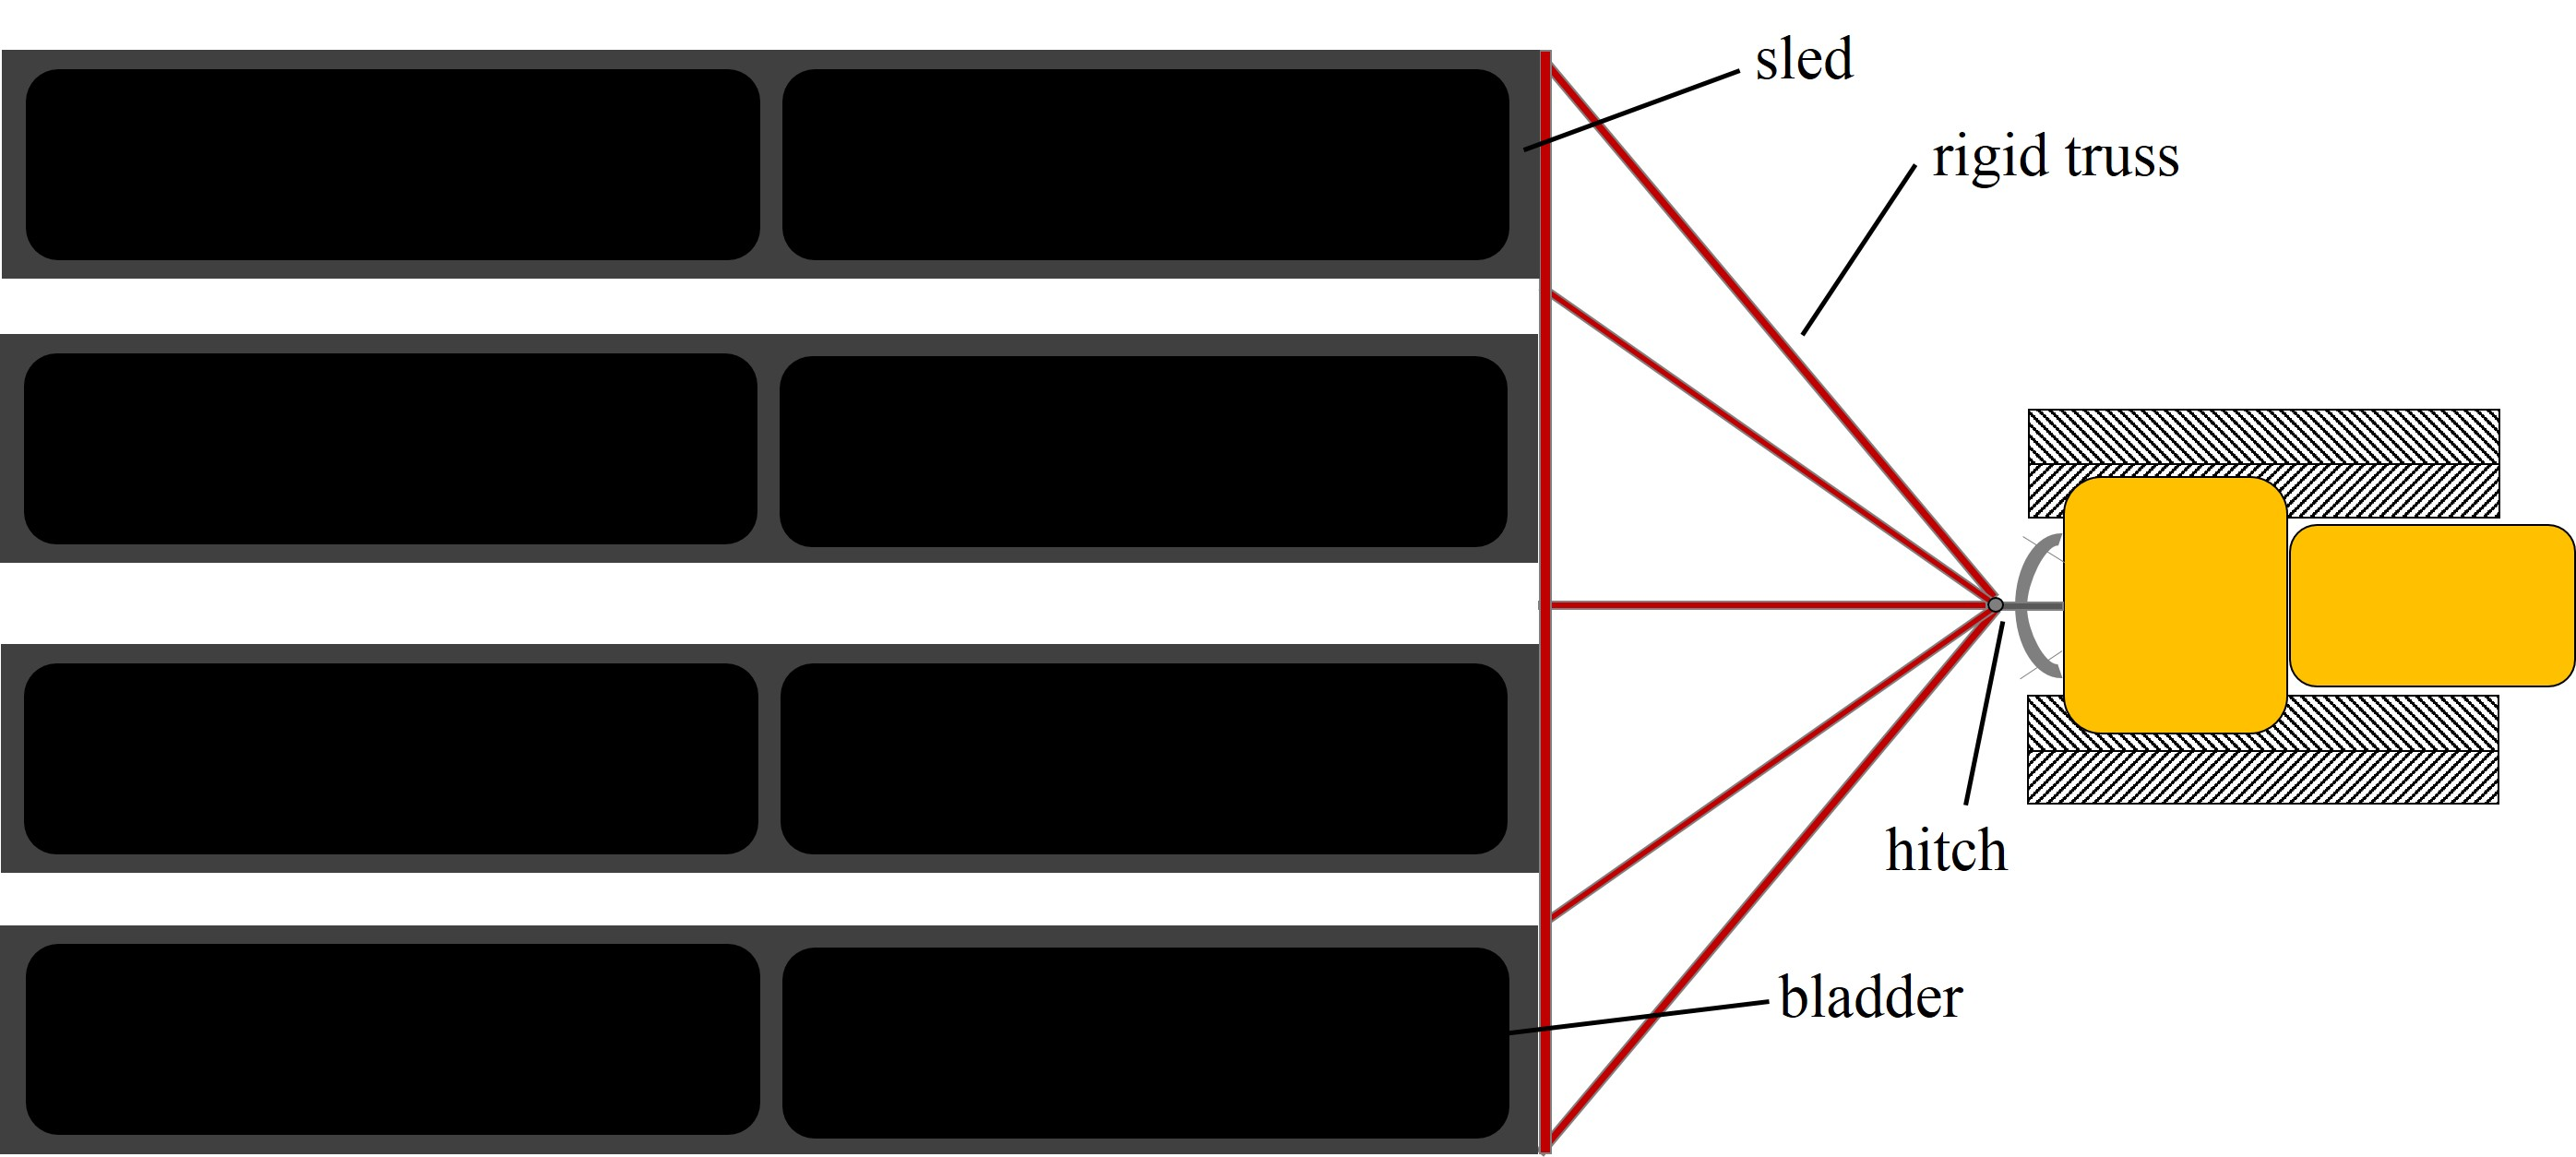
\includegraphics[width=4in]{Top_View_Diagram_South_Pole_Traverse}
    \caption{Diagram of the South Pole Traverse tractor-sled towing configuration. Sleds are attached to the rigid, red truss where fuel bladders rest on top. The red truss inserts at the drawbar hitch of the tractor.}
    \label{fig:Top_View_Diagram_South_Pole_Traverse}
\end{figure} 
Documentation and data for the tractor and sled system can be found in \cite{lever2012high, Caterpillar2002}.